\documentclass[twoside,a4paper]{master}
\usepackage[kerning,spacing]{microtype}
\usepackage{float}
\usepackage{booktabs}
% Math support (provides \text and other commands used in formulas)
\usepackage{amsmath}
\usepackage{siunitx}
\usepackage{makecell}
\DeclareSIUnit{\angstrom}{\text{\AA}}
\usepackage{subcaption}
% Relax line breaking to avoid overfull boxes from long code/paths
\emergencystretch=2em
% Quiet certain deprecated KOMA-Script interface warnings
\usepackage{scrhack}
% Acronyms & glossary (no external makeglossaries needed)
\usepackage[acronym]{glossaries}
\hypersetup{hidelinks}


\microtypecontext{spacing=nonfrench}

% Helpfull command to put reminders in your work
\newcommand{\Todo}[1]%
{\fcolorbox{black}{orange}{\parbox{\dimexpr\textwidth-2\fboxsep-2\fboxrule}{\textbf{Todo: #1}}}}
% it uses one argument which is referred to by #1

\newcommand{\Alphabet}{\mathcal{A}\xspace}

% Add bibliography resource
\addbibresource{references.bib}

\makenoidxglossaries

\newacronym{lev}{LEV}{local environment validation}
\newacronym{tcs}{TCS}{transplant clash score}
\newacronym{rmsd}{RMSD}{root-mean-square deviation}
\newacronym{pdb}{PDB}{Protein Data Bank}
\newacronym{rcsbpdb}{RCSB PDB}{Research Collaboratory for Structural Bioinformatics Protein Data Bank}
\newacronym{api}{API}{application programming interface}
\newacronym{atp}{ATP}{adenosine triphosphate}
\newacronym{adp}{ADP}{adenosine diphosphate}
\newacronym{fad}{FAD}{flavin adenine dinucleotide}
\newacronym{fmn}{FMN}{flavin mononucleotide}
\newacronym{nad}{NAD}{nicotinamide adenine dinucleotide}
\newacronym{nadh}{NADH}{nicotinamide adenine dinucleotide (reduced)}
\newacronym{nadph}{NADPH}{nicotinamide adenine dinucleotide phosphate (reduced)}
\newacronym{plp}{PLP}{pyridoxal 5'-phosphate}
\newacronym{nmr}{NMR}{nuclear magnetic resonance}
\newacronym{cryoem}{cryo-EM}{cryogenic electron microscopy}
\newacronym{http}{HTTP}{hypertext transfer protocol}
\newacronym{url}{URL}{uniform resource locator}
\newacronym{json}{JSON}{JavaScript Object Notation}
\newacronym{html}{HTML}{HyperText Markup Language}
\newacronym{pdf}{PDF}{Portable Document Format}
\newacronym{sdf}{SDF}{structure data file}
\newacronym{edf}{EDF}{extended descriptor file}
\newacronym{xml}{XML}{eXtensible Markup Language}
\newacronym{peg}{PEG}{polyethylene glycol}
\newacronym{mpd}{MPD}{2-methyl-2,4-pentanediol}
\newacronym{gol}{GOL}{glycerol}
\newacronym{edo}{EDO}{1,2-ethanediol}
\newacronym{sam}{SAM}{S-adenosyl methionine}
\newacronym{sah}{SAH}{S-adenosyl homocysteine}
\newacronym{ec}{EC}{Enzyme Commission}
\newacronym{ccd}{CCD}{Chemical Component Dictionary}
\newacronym{wwpdb}{wwPDB}{worldwide Protein Data Bank}
\newacronym{uml}{UML}{Unified Modeling Language}
\newacronym{ci}{CI}{confidence interval}
\newacronym{vdw}{vdW}{van der Waals}
\newacronym{plddt}{pLDDT}{predicted local distance difference test}
\newacronym{cc}{CC}{Creative Commons}
\newacronym{het}{HET}{heteroatom}
\newacronym{dog}{DoG}{difference of Gaussians}
\newacronym{uniprot}{UniProt}{Universal Protein Resource}
\newacronym{rest}{REST}{Representational State Transfer}
\newacronym{bfgs}{BFGS}{Broyden-Fletcher-Goldfarb-Shanno}
\newacronym{lslbfgs}{LSL-BFGS}{Line-Search Limited-memory Broyden-Fletcher-Goldfarb-Shanno}

\begin{document}

% use roman page numbers before the real document starts.
\pagenumbering{roman}

%Change the values here to get your title page and assertion page right
\AdvisorA{Prof. Dr. Matthias Rarey}
\AdvisorB{Prof. Dr. Andrew Torda}
\author{Marius R\"uve}
\MatrikelNo{7657327}
%\AuthorAdress{Musterstrasse 1}{07770 M\"unchhausen}
\title{
  \begin{tabular}{c}
    \textbf{Ligand Transplantation and Optimization} \\[3mm]
    \textbf{in Protein Models}
  \end{tabular}}
\Maketitle

% !TEX root = ../main.tex
\addchap*{Abstract}
\small
Protein structure prediction now spans entire proteomes, yet most AlphaFold models lack bound ligands and cofactors. This work builds and evaluates a reproducible pipeline that enriches AlphaFold monomers through DoGSite3 pocket detection, SIENA donor retrieval and alignment, ligand extraction, transplantation, and optional JAMDAscorer pose-only refinement. Three site-centric indicators are reported: local RMSD, TCS, and LEV, with a shared success gate of local RMSD $\leq$ \SI{1.0}{\angstrom} and TCS $\leq 0.35$ while LEV remains descriptive.

On a stratified benchmark of \num{2370} targets, \num{1840} yielded at least one placement, producing \num{6658} post-JAMDAscorer placements with a median of two per completed target. The joint gate retained \num{3592} placements (\SI{54.0}{\percent}) across \num{1457} targets, and LEV was defined for \num{6004} of \num{6658} placements overall and \num{5860} of \num{6488} organic placements. External benchmarking identified \num{2496} shared placements with AlphaFill; among the \num{1372} pairs where both Local RMSD and TCS were defined, pass rates were \SI{62.9}{\percent} (\num{863}/\num{1372}) for this pipeline and \SI{88.9}{\percent} (\num{1220}/\num{1372}, 95\%\,CI: 87.2--90.5) for AlphaFill, with moderate correlation in TCS and weaker alignment on local RMSD. Median wall times from instrumented runs were \SI{0.94}{\second} for DoGSite3, \SI{0.45}{\second} for SIENA, \SI{0.41}{\second} for JAMDAscorer, and \SI{6.0}{\second} per target overall, demonstrating scalable enrichment. Brief ablations indicate limited benefit from tightening the active-site identity threshold beyond 0.85, so the combined gate highlights residual errors from pocket-state mismatches, metal coordination differences, and low-identity outliers.

\normalsize


\setcounter{tocdepth}{1}
\tableofcontents
\clearpage
\listoffigures
\clearpage
\listoftables
\clearpage
\printnoidxglossary[type=\acronymtype]
\clearpage

% List of acronyms
\pagenumbering{arabic}

\include{chapters/01_introduction}
\include{chapters/02_methods}
\include{chapters/03_results}
\chapter{Conclusion}
\label{chap:conclusion}

\section{Conclusion}
This thesis evaluates a site-centric pipeline that transplants ligands into AlphaFold monomers by combining DoGSite3 pocket detection, SIENA pocket alignment, ligand extraction and placement, optional JAMDAscorer refinement, and three complementary indicators of placement quality: Local \gls{rmsd}, the \gls{tcs}, and the \gls{lev}.

\subsection*{Answers to the Research Questions}
\paragraph{RQ1: What placement quality and coverage does the pipeline achieve on AlphaFold monomers?} Across \num{2370} configured targets, \num{1840} monomers yield at least one ligand placement for a total of \num{6658} post-refinement hypotheses. Applying the joint success gate (local \gls{rmsd} $\leq$ \SI{1.0}{\angstrom} and \gls{tcs} $\leq 0.35$) retains \num{3592} placements across \num{1457} proteins, equal to \SI{54.0}{\percent} of the refined set (Table~\ref{tab:attrition-funnel}, Table~\ref{tab:overall-summary}, and Table~\ref{tab:internal-success}). Median post-refinement scores are \SI{0.386}{\angstrom} for local \gls{rmsd} and 0.263 for \gls{tcs}, highlighting that near-native poses dominate the retained cohort (Table~\ref{tab:global-quality-stats}). \gls{lev} is defined for \num{6004} placements overall (\num{5860} organic) and augments the clash metric by tracing local backbone deviations (Section~\ref{sec:results-quality}).

\paragraph{RQ2: Which configuration choices are supported by the ablations?} Identity sweeps indicate that a SIENA site-identity threshold near $0.85$ preserves yield while suppressing clear outliers; tightening the cutoff beyond this value yields diminishing returns (Section~\ref{sec:results-ablations}). Excluding monoatomic ions from the \gls{tcs} calculation reduces false clashes without materially altering the joint pass rate. JAMDAscorer systematically lowers \gls{tcs} with negligible pose movement (median $\Delta$Local RMSD $\approx$ \SI{0.00}{\angstrom}), confirming its role as a geometry clean-up stage rather than a re-docking surrogate (Section~\ref{sec:results-optimization} and Table~\ref{tab:jamda-deltas}). The recommended defaults are: SIENA identity $\approx 0.85$; success gate local \gls{rmsd} $\leq$ \SI{1.0}{\angstrom} and \gls{tcs} $\leq 0.35$; and ions excluded from the \gls{tcs} tally.

\paragraph{RQ3: How does the pipeline compare with AlphaFill on the matched cohort?} The benchmarking identified \num{2496} overlapping placements. Among the \num{1372} pairs where both local \gls{rmsd} and \gls{tcs} were defined, AlphaFill achieves lower medians and a higher joint pass rate (\SI{88.9}{\percent}, \num{1220}/\num{1372}, 95\%\,CI: 87.2--90.5) than this pipeline (\SI{62.9}{\percent}, \num{863}/\num{1372}). Cross-pipeline correlations remain moderate, suggesting that donor selection and refinement strategies drive the observed differences (Section~\ref{sec:results-external}, Table~\ref{tab:ff-af-success}, and Table~\ref{tab:ff-af-corr}).

\subsection*{Implications}
Large-scale ligand enrichment of AlphaFold monomers is feasible at single-digit seconds per target while preserving measurable quality under the strict geometric-and-clash gate. The orthogonal error modes captured by local \gls{rmsd}, \gls{tcs}, and \gls{lev} reinforce the value of the joint gate for reporting: Figure~\ref{fig:cross-metric} shows limited cross-metric correlation, and Figures~\ref{fig:failure_modes_case_studies:success},~\ref{fig:failure_modes_case_studies:collapsed}, and~\ref{fig:failure_modes_case_studies:metal} (Appendix~\ref{app:supp-figs}) highlight the complementary failure signatures. Together, these results motivate publishing placement sets with all three metrics to guide downstream interpretation.

\subsection*{Limitations}
The workflow deliberately targets non-polymer ligands and metal ions commonly represented in the \gls{rcsbpdb}. It does not perform full flexible-receptor docking or quantum refinement, nor does it attempt to model post-translational modifications or glycans. As with any homology-based approach, transplant reliability depends on the availability and quality of structurally similar donors and their conformational compatibility with the AlphaFold receptor. The enriched models should therefore be interpreted as \emph{qualitative} hypotheses that can prioritize experiments or heavier simulations rather than as quantitatively precise holo structures \cite{hekkelmanAlphaFillEnrichingAlphaFold2023}.

Primary failure modes include pocket-state mismatches between donors and receptors, metal-site mis-coordination, and low-identity alignments that still clear the threshold yet distort local geometry (Section~\ref{sec:results-failure-modes}). \gls{lev} requires a suitable donor reference, rendering it unavailable for a subset of placements, and the current clash evaluation omits hydrogen bonding, electrostatics, and protonation mismatches that may matter for detailed modelling. Runtime estimates also exclude the cost of donor curation and external data refreshes.

\subsection*{Recommendations and Future Work}
\begin{itemize}
    \item Adopt the recommended defaults from RQ2 and report both single-metric and joint-gate outcomes to maintain alignment with prior analyses.
    \item Add metal-aware handling and rotameric sampling for coordinating residues to address the dominant clash-heavy failure class observed in Section~\ref{sec:results-failure-modes}.
    \item Expand donor selection with multi-template consensus and sequence-environment weighting to suppress outliers that stem from marginal alignments.
    \item Incorporate pocket-state classification and, where available, AlphaFold model ensembles to mitigate state mismatches for flexible sites.
    \item Re-evaluate the workflow against updated structure predictors and external enrichment resources as they emerge to track field-level progress.
\end{itemize}

\section{Concluding Remarks}
Homology-guided ligand transplantation, combined with lightweight JAMDAscorer refinement and orthogonal quality checks, provides a practical route to convert apo AlphaFold models into context-rich hypotheses at scale. The workflow is robust enough to support downstream design while signalling when placements warrant caution, charting clear directions for targeted refinements and broader dissemination.


\newpage
\small
% Bibliography using biblatex
\printbibliography[title=References]
\normalsize

% appendix

\appendix
\noappendicestocpagenum
\addappheadtotoc

% !TEX root = ../main.tex
\chapter{Reproducibility Details}\label{app:reproducibility}
\noindent\fbox{\parbox{0.97\linewidth}{\textbf{Code Availability.} The pipeline implementation is available at \url{https://github.com/mariusrueve/foldfusion}.}}

All experiments were executed on a Linux workstation with Python-based orchestration and locally installed DoGSite3, SIENA, LigandExtractor, and JAMDAscorer binaries. The runs used Ubuntu~24.04.3~LTS (Linux kernel~6.14.0-29-generic) on an AMD~Ryzen~7~7800X3D CPU with \SI{32}{\giga\byte} RAM, paired with an NVIDIA~GeForce~RTX~4070 discrete GPU (GNOME~46 on X11). Detailed operational instructions, including environment preparation, exact commands, and configuration snapshots, are provided in the accompanying documentation.

\paragraph{FoldFusion codebase.}
\begin{itemize}
    \item Project version: \texttt{foldfusion==0.1.0} (editable install)
    \item Python interpreter: CPython~3.12.3 within a virtual environment created via \texttt{python3 -m venv}
    \item pip version: \texttt{pip~24.0}
\end{itemize}

\paragraph{External executables.}
\begin{itemize}
    \item DoGSite3~1.1.0 \hfill (\texttt{/home/marius/Data/zbh/dogsite3\_1.1.0/dogsite3})
    \item SIENA~1.3.0 \hfill \makecell[l]{(\texttt{/home/marius/Data/zbh/siena\_1.3.0/siena}\\and \texttt{generate\_siena\_database})}
    \item LigandExtractor~2025-04 \hfill \makecell[l]{(\texttt{/home/marius/Data/zbh/}\\\texttt{LigandExtractor\_2025-04/ligand\_extractor})}
    \item JamdaScorer~1.0.0 \hfill (\texttt{/home/marius/Data/zbh/JamdaScorer\_1.0.0/JamdaScorer})
\end{itemize}

\paragraph{Python package stack (pip freeze).}
The following dependency snapshot was captured inside the project virtual environment immediately after the thesis experiments:

\begin{verbatim}
certifi==2025.8.3
charset-normalizer==3.4.3
contourpy==1.3.3
coverage==7.10.6
cycler==0.12.1
-e git+https://github.com/mariusrueve/foldfusion.git@
    9b5368810c268f79f19d92ba930f9485adbea2dc#egg=foldfusion
fonttools==4.60.0
idna==3.10
iniconfig==2.1.0
Jinja2==3.1.6
kiwisolver==1.4.9
MarkupSafe==3.0.2
matplotlib==3.10.6
mypy==1.18.1
mypy_extensions==1.1.0
narwhals==2.5.0
numpy==2.3.3
numpy-typing-compat==20250818.2.3
optype==0.13.4
packaging==25.0
pandas==2.3.2
pandas-stubs==2.3.2.250827
pathspec==0.12.1
pillow==11.3.0
plotly==6.3.0
pluggy==1.6.0
Pygments==2.19.2
pyparsing==3.2.4
pytest==8.4.2
pytest-cov==7.0.0
python-dateutil==2.9.0.post0
pytz==2025.2
requests==2.32.5
ruff==0.13.0
scipy==1.16.2
scipy-stubs==1.16.2.0
seaborn==0.13.2
six==1.17.0
tqdm==4.67.1
types-pytz==2025.2.0.20250809
types-requests==2.32.4.20250913
typing_extensions==4.15.0
tzdata==2025.2
urllib3==2.5.0
\end{verbatim}

The editable installation line documents the exact repository commit used for the experiments; package versions inherit the numbering emitted by \texttt{pip freeze}. When reproducing the pipeline, installing the dependencies above inside CPython~3.12.3 together with the listed external binaries suffices to recover the environment that produced the reported figures and tables.

Figure~\ref{fig:stage-runtime} summarizes per-stage runtimes for a stratified sample of \num{303} targets drawn from the production run (every eighth UniProt in lexicographic order). The distributions confirm that DoGSite3, SIENA, and JAMDAscorer remain within seconds per target under the hardware setup described above.

\begin{figure}[ht]
    \centering
    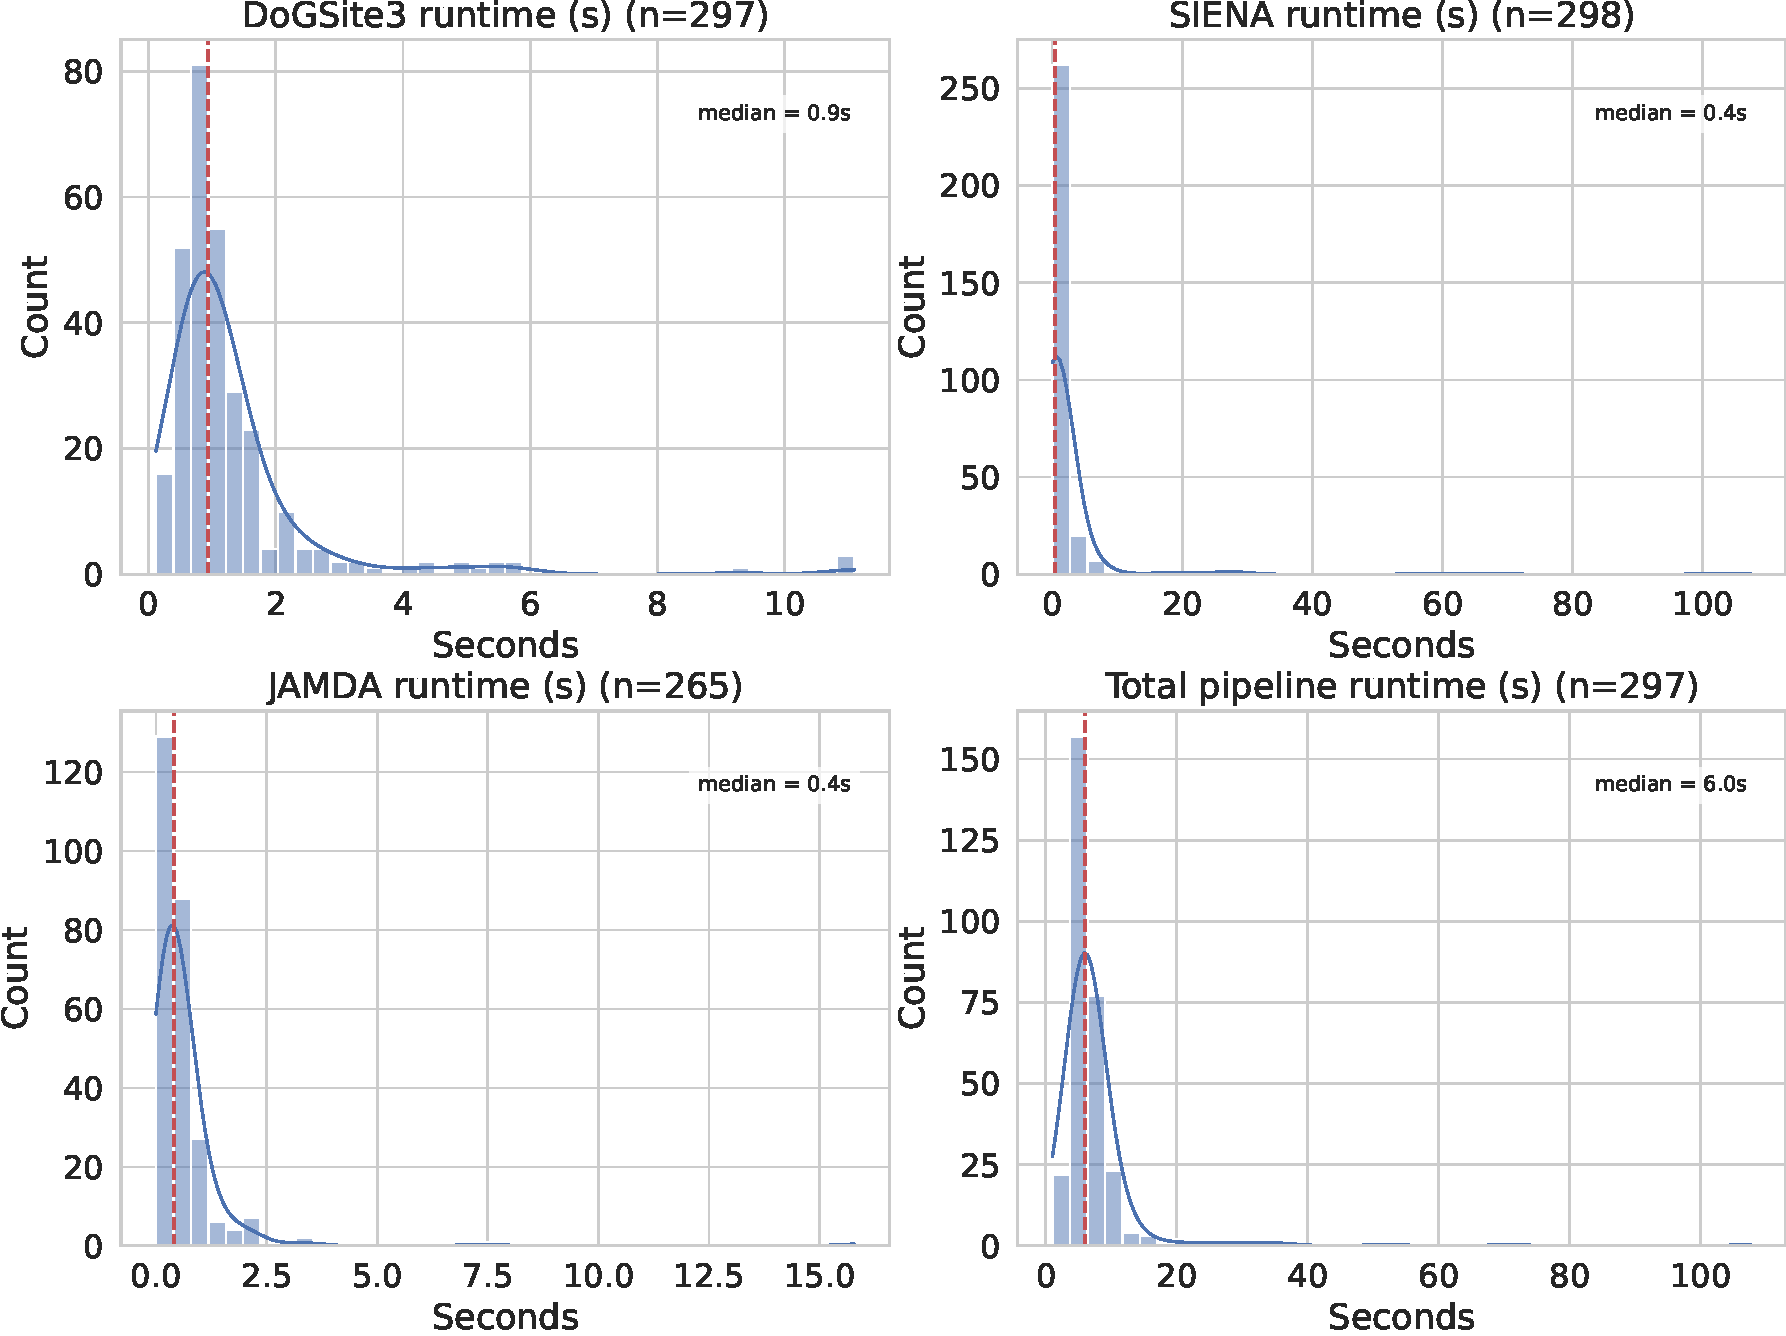
\includegraphics[width=0.9\linewidth]{figures/03_results/fig_stage_runtime_histograms.pdf}
    \caption[Stage runtime distributions]{Per-stage wall-time distributions across the \num{303}-target monitoring sample captured via stage-specific instrumentation. Vertical dashed lines mark medians, and sample sizes differ because DoGSite3 logs once per target, SIENA only when a donor aligns, and JAMDAscorer only when a placement is optimized.}
    \label{fig:stage-runtime}
\end{figure}

Table~\ref{tab:appendix-ion-breakdown} reports the ligand-class breakdown for the \num{6658} post-JAMDAscorer placements where \gls{tcs} metrics are defined. Monoatomic ions are counted separately because they are excluded from clash scoring, yielding \num{6488} organic placements (\SI{97.4}{\percent}) and \num{170} monoatomic ions (\SI{2.6}{\percent}) consistent with the Results chapter.

\begin{table}[ht]
\centering
\resizebox{\linewidth}{!}{%
\begin{tabular}{lrll}
\toprule
Category & Placements & Fraction & Notes \\
\midrule
Organic / polyatomic ligands & 6488 & \SI{97.4}{\percent} & Valid \gls{tcs} and \gls{lev} metrics available when donors provide references \\
Monoatomic ions & 170 & \SI{2.6}{\percent} & \gls{tcs} excluded from the main statistics; reported separately in plots \\
\bottomrule
\end{tabular}
}
\caption[Ligand class distribution]{Ligand-class distribution for the post-JAMDAscorer placements with defined \gls{tcs} metrics. Totals exclude cases where ligand extraction failed (none in the final run).}
\label{tab:appendix-ion-breakdown}
\end{table}


Licensing summary: DoGSite3 and SIENA are distributed for non-commercial academic research by the ZBH/University of Hamburg. JAMDAscorer is licensed for research use only. AlphaFold DB structures are provided under CC-BY~4.0, and mirrored PDB entries fall under the wwPDB data-use policy. Derived models should therefore be redistributed only with attribution to all upstream sources.

% !TEX root = ../main.tex
\chapter{Supplementary Figures}\label{app:supp-figs}
Additional figures referenced in the main text are collated here for completeness.

\begin{figure}[ht]
    \centering
    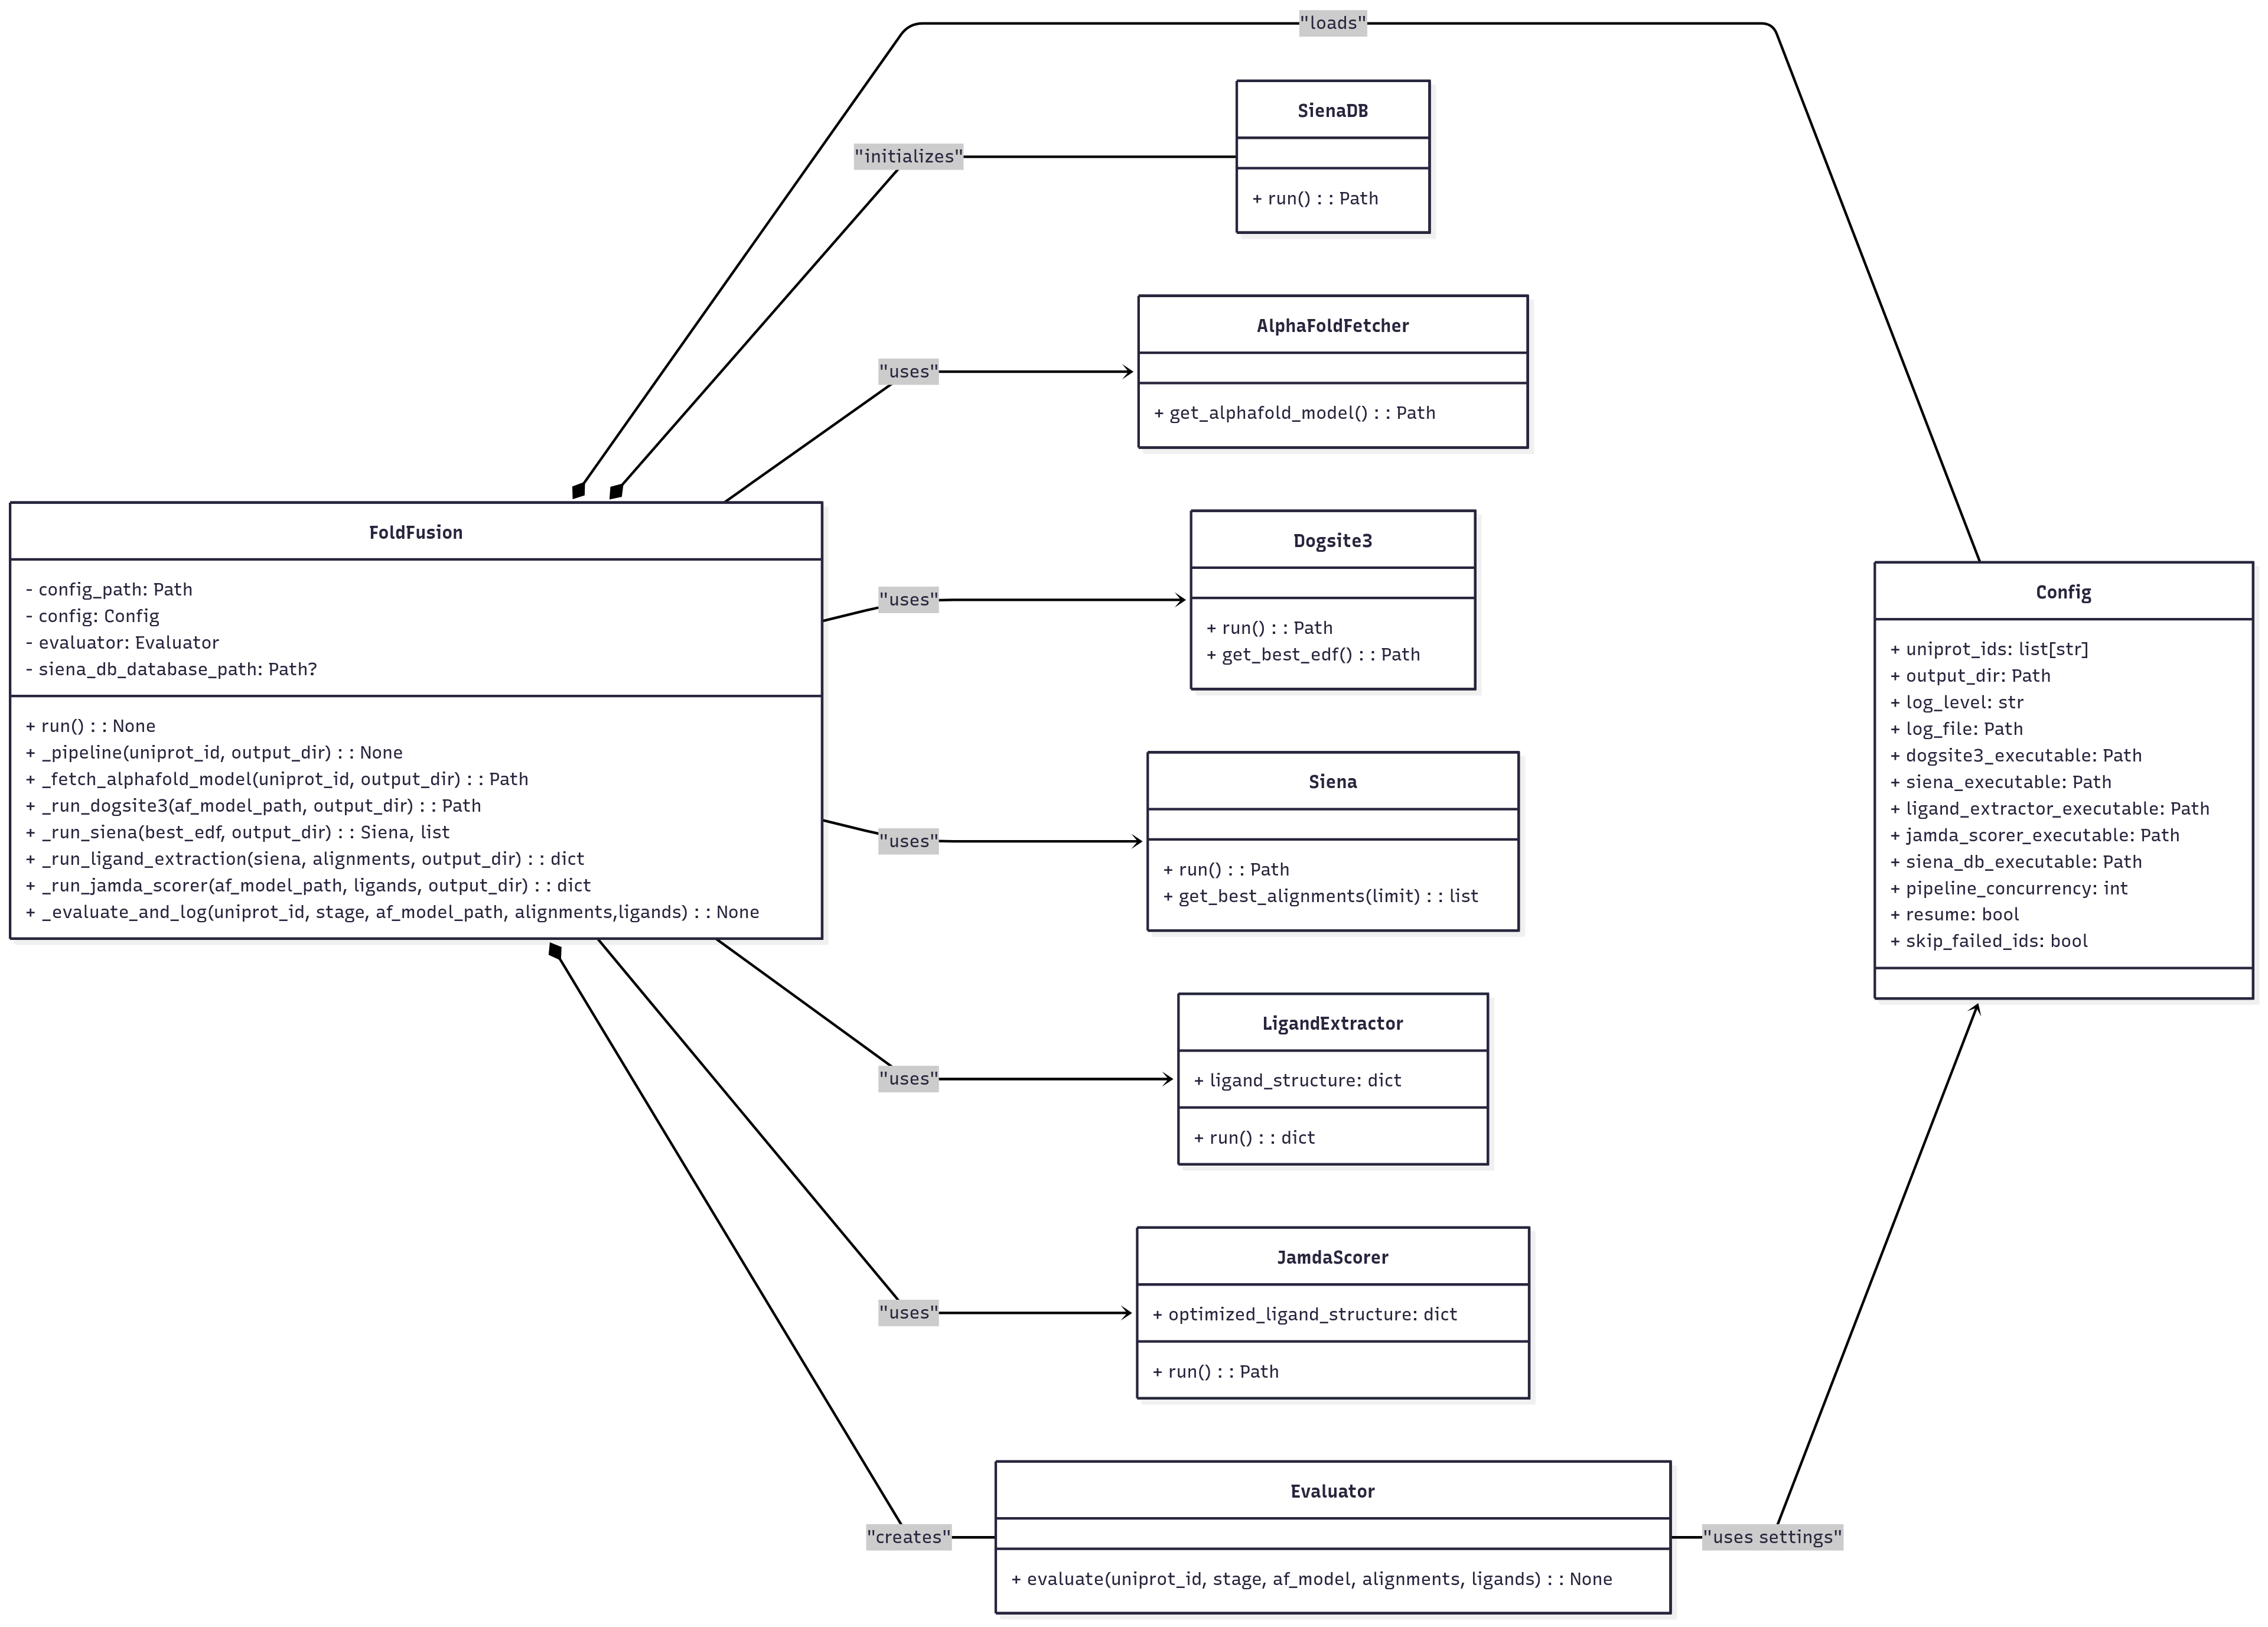
\includegraphics[width=0.95\linewidth]{figures/foldfusion_pipeline_uml.png}
    \caption[Pipeline UML overview]{UML class diagram of the pipeline. The central orchestrator coordinates data fetching, pocket detection, donor alignment, ligand extraction, scoring, and evaluation via the surrounding tool adapters and configuration object. Node labels retain the \texttt{FoldFusion} class name used in the code to denote this work's pipeline implementation.}
    \label{fig:pipeline_overview_uml}
\end{figure}

% Failure mode case studies — enlarged single-panel figures moved from main text
\begin{figure}[ht]
    \centering
    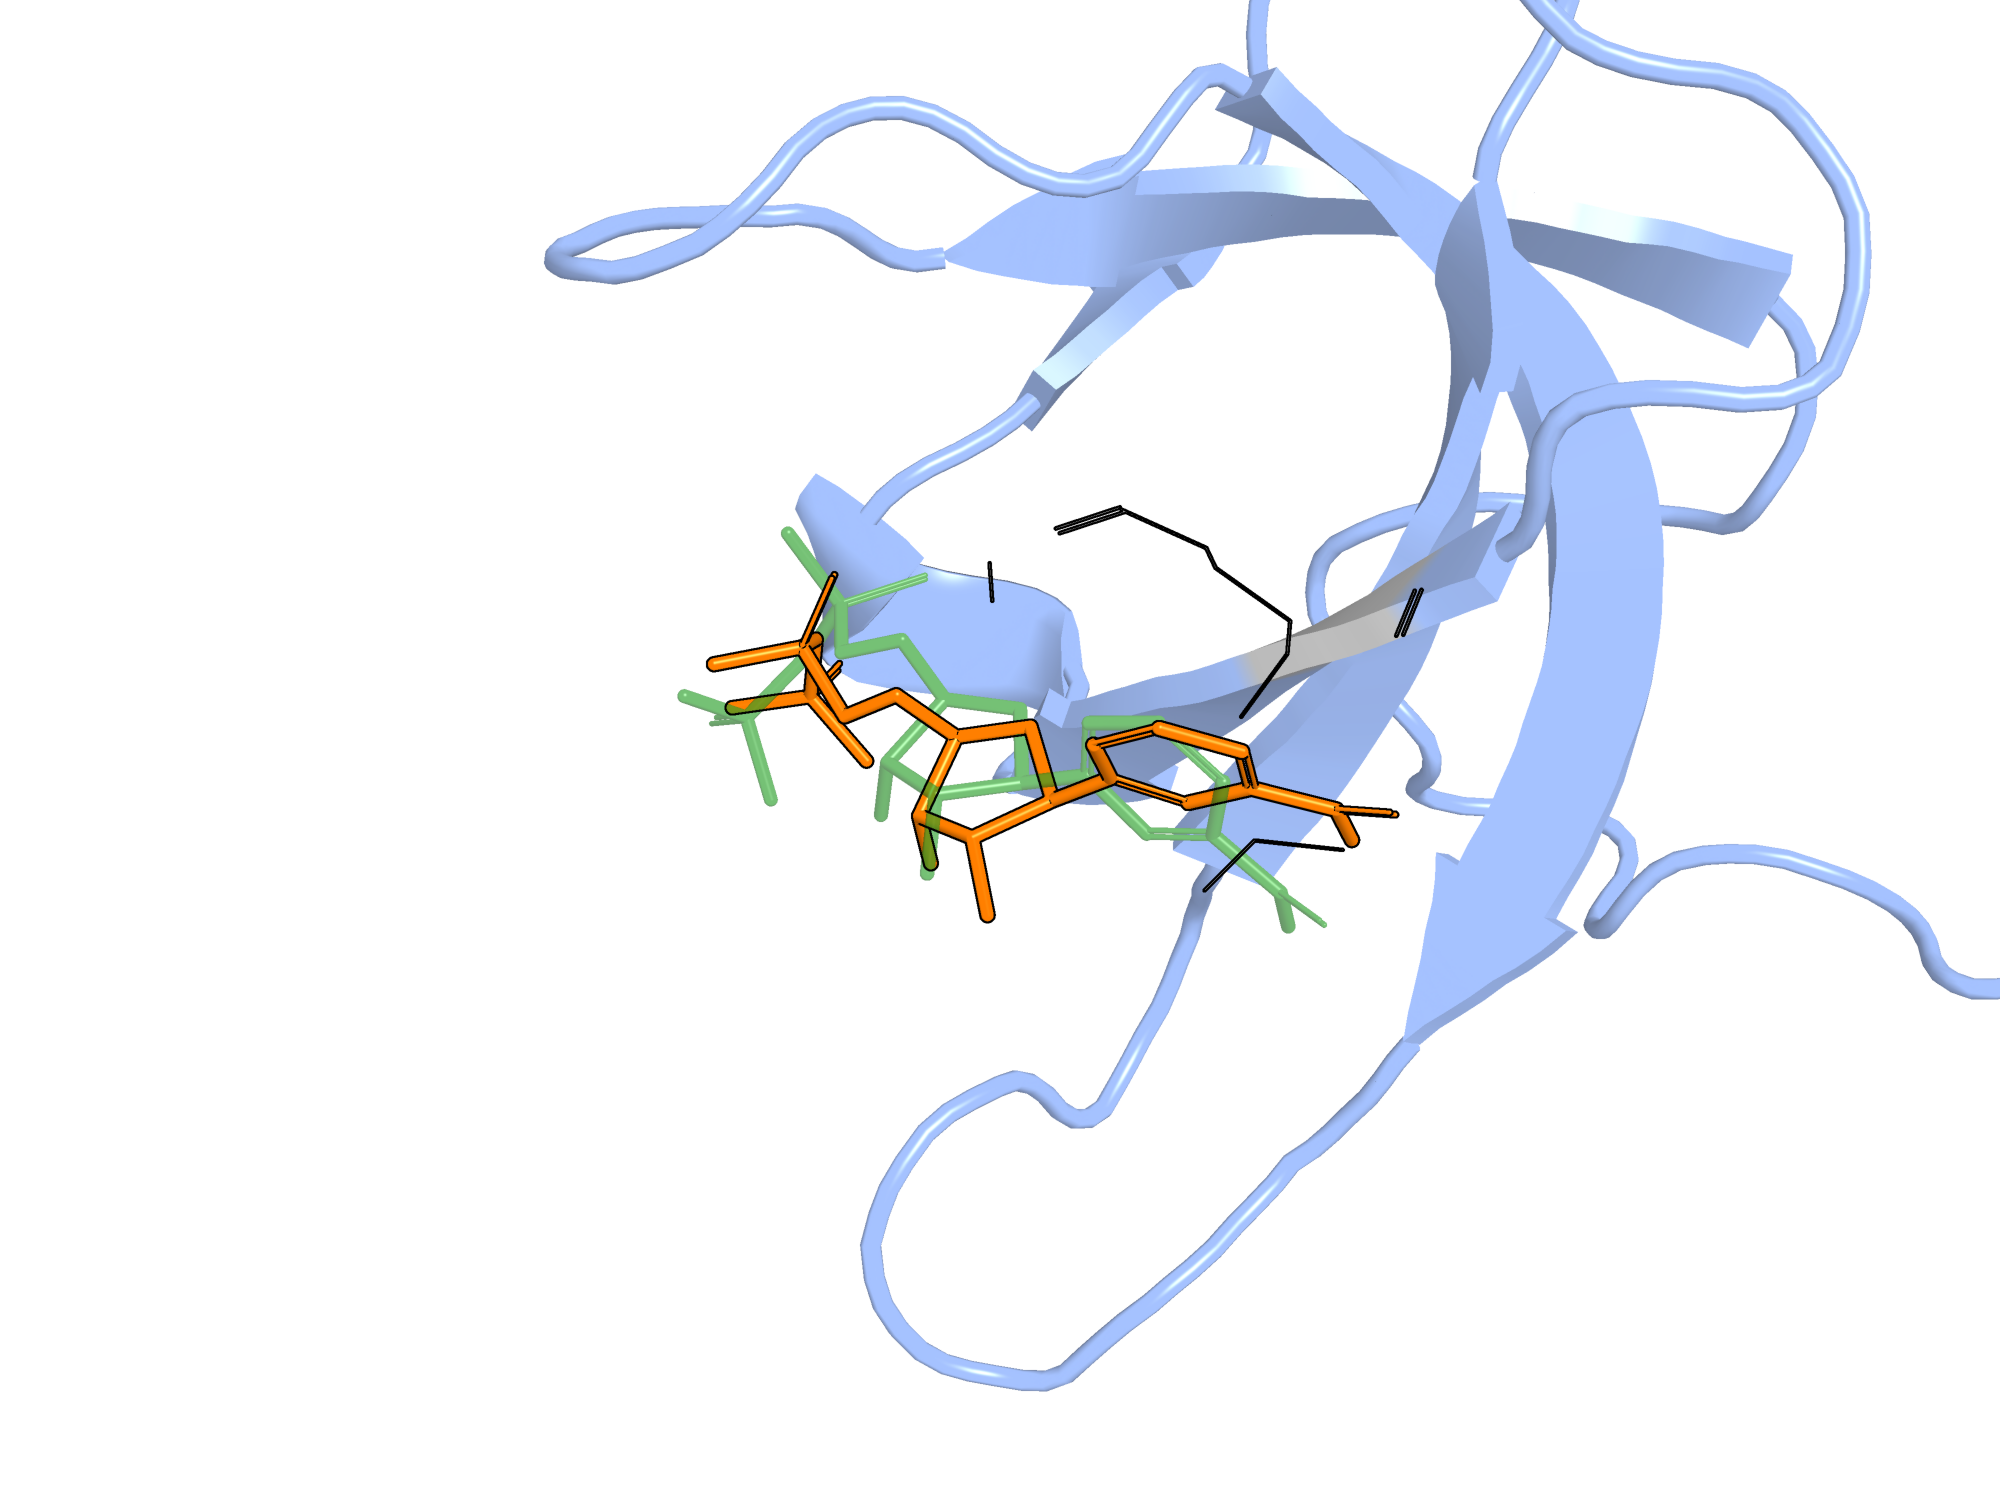
\includegraphics[width=0.85\linewidth]{figures/foldfusion_P00383_success_iso.png}
    \caption[Reference success case]{Reference success case (green: donor, orange: refined). Rendered with PyMOL~\cite{PyMOL, AxPyMOL}.}
    \label{fig:failure_modes_case_studies:success}
\end{figure}

\begin{figure}[ht]
    \centering
    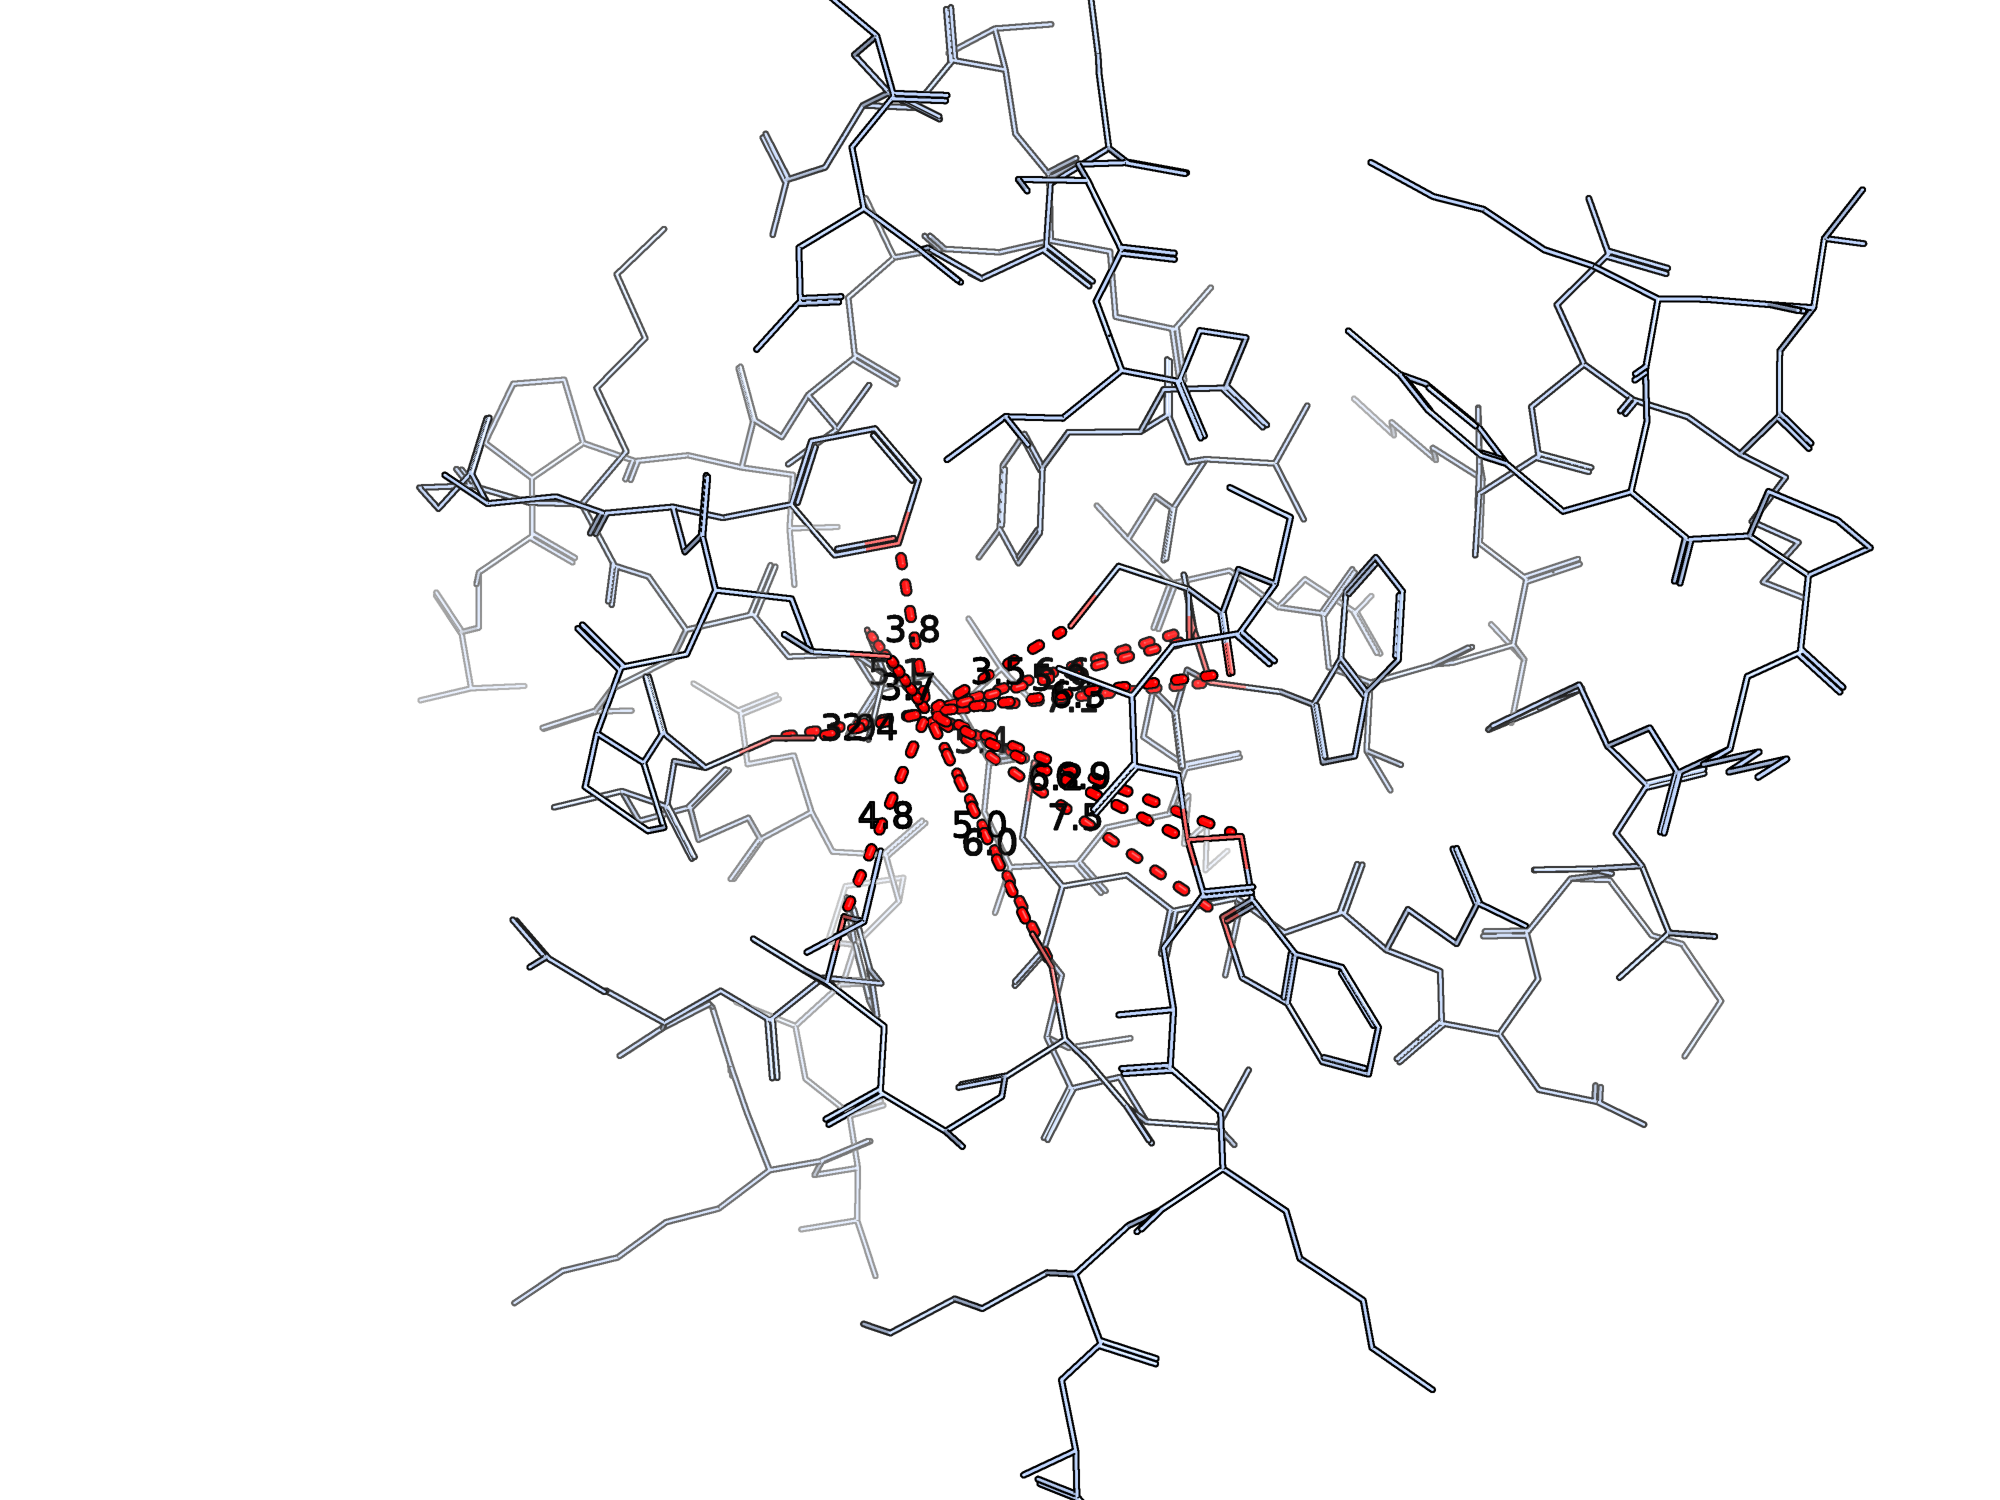
\includegraphics[width=0.85\linewidth]{figures/foldfusion_P80882_failure.png}
    \caption[Collapsed-loop failure]{Collapsed-loop failure example. Rendered with PyMOL~\cite{PyMOL, AxPyMOL}.}
    \label{fig:failure_modes_case_studies:collapsed}
\end{figure}

\begin{figure}[ht]
    \centering
    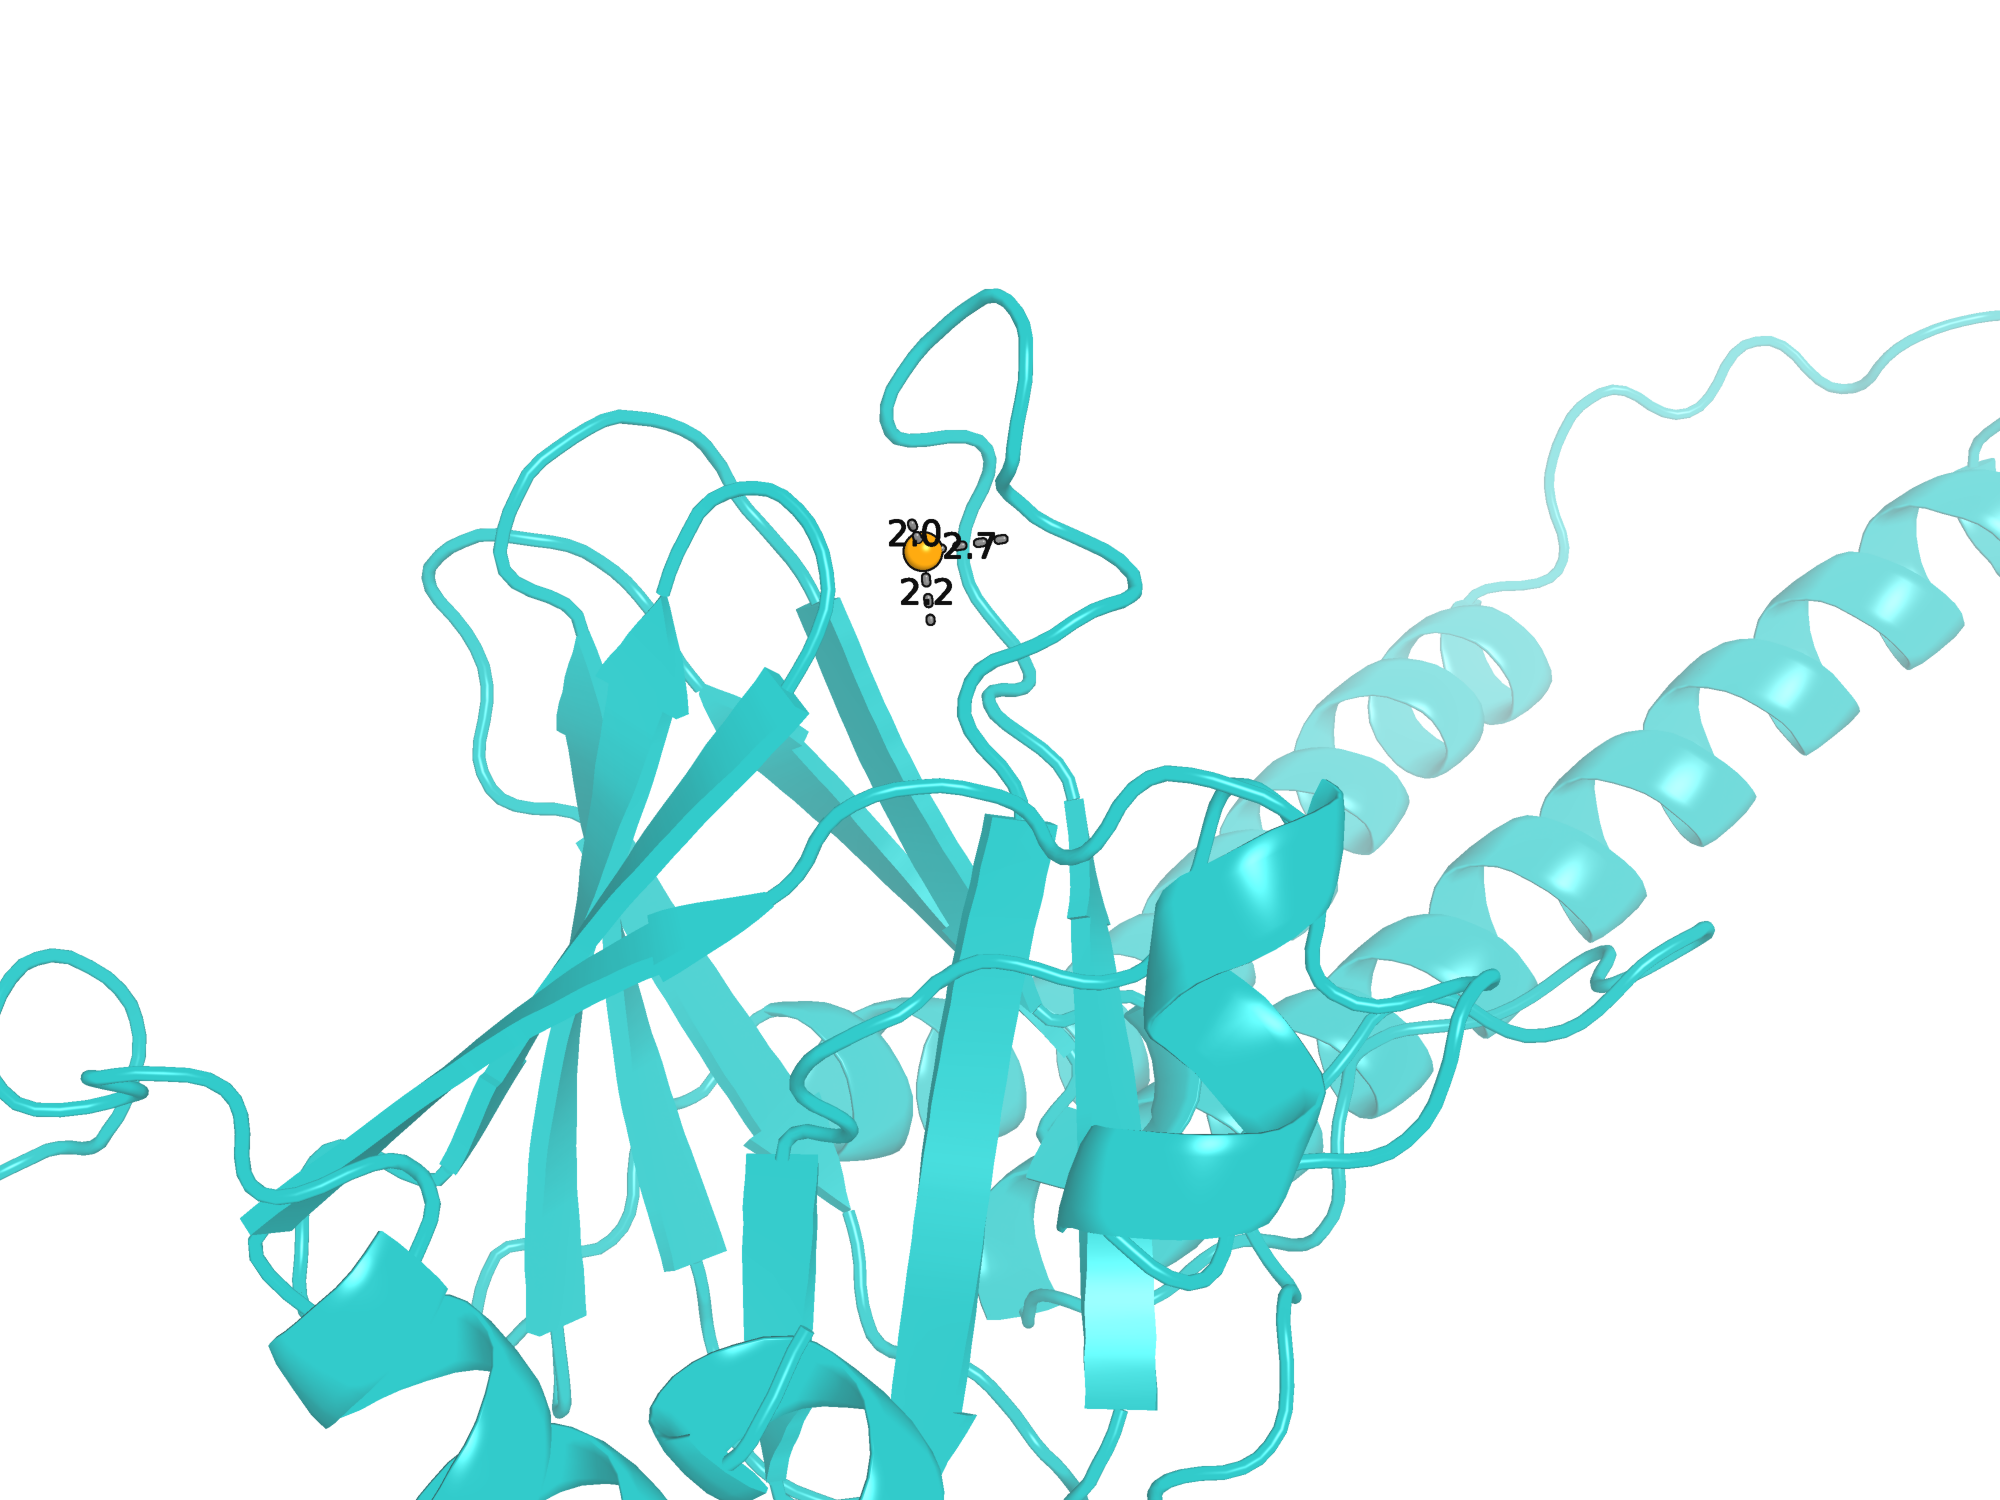
\includegraphics[width=0.85\linewidth]{figures/foldfusion_P08306_metal.png}
    \caption[Metal mis-coordination failure]{Metal mis-coordination failure example. Rendered with PyMOL~\cite{PyMOL, AxPyMOL}.}
    \label{fig:failure_modes_case_studies:metal}
\end{figure}

\begin{figure}[ht]
    \centering
    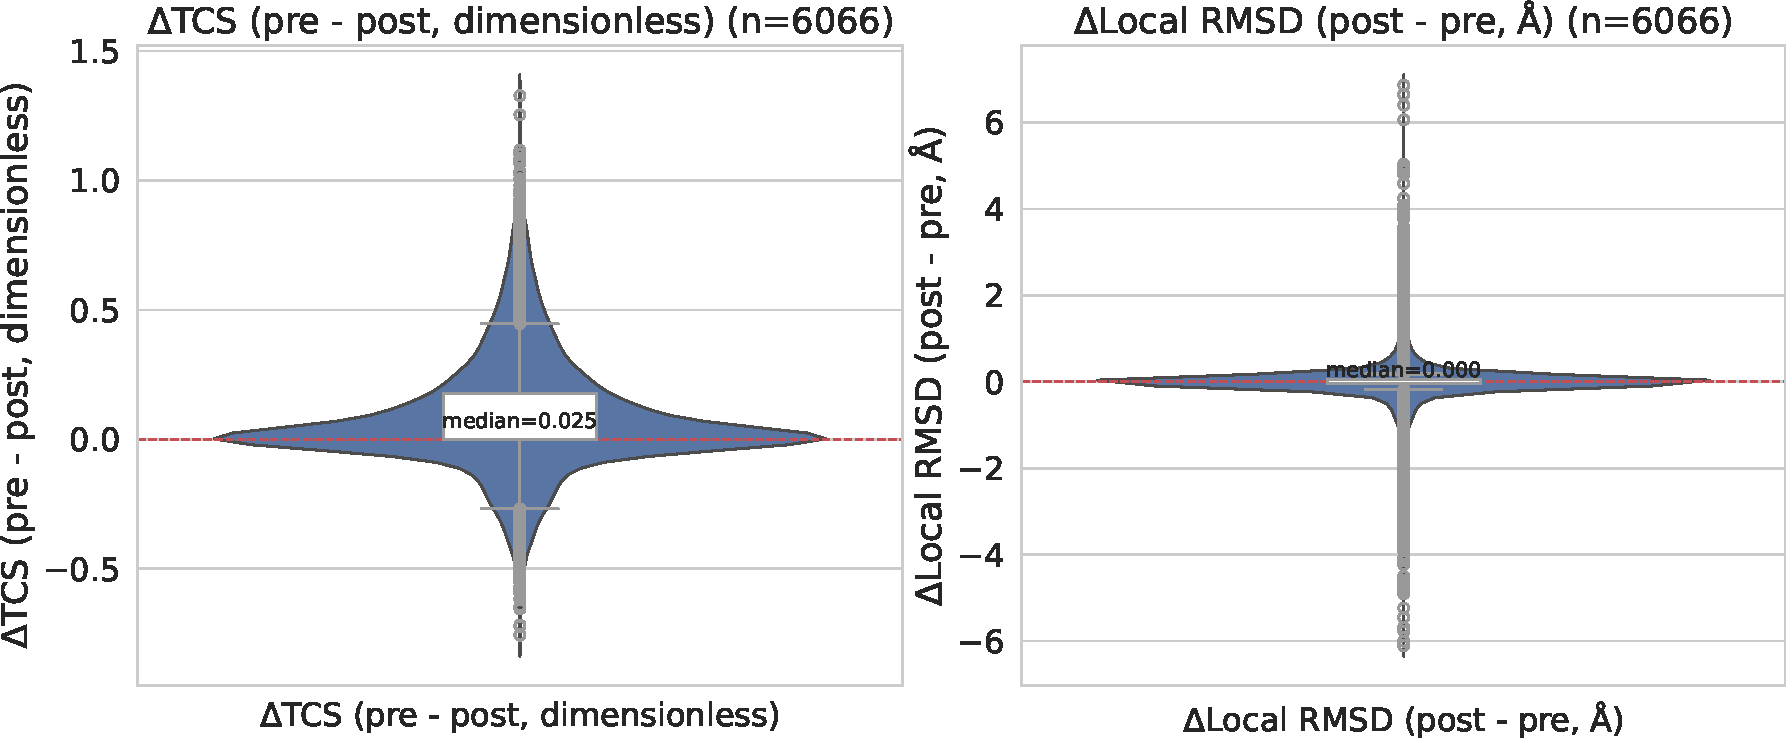
\includegraphics[width=0.85\linewidth]{figures/03_results/fig_jamda_delta_distributions.pdf}
    \caption[JAMDAscorer delta distributions]{Distributions of paired JAMDAscorer deltas ($\Delta$\gls{tcs} and $\Delta$local \gls{rmsd}) for the \num{6066} placements that produced both pre- and post-optimization metrics. Zero indicates no change, and negative $\Delta$\gls{tcs} denotes fewer clashes after optimization.}
    \label{fig:jamda-deltas}
\end{figure}

\begin{figure}[ht]
    \centering
    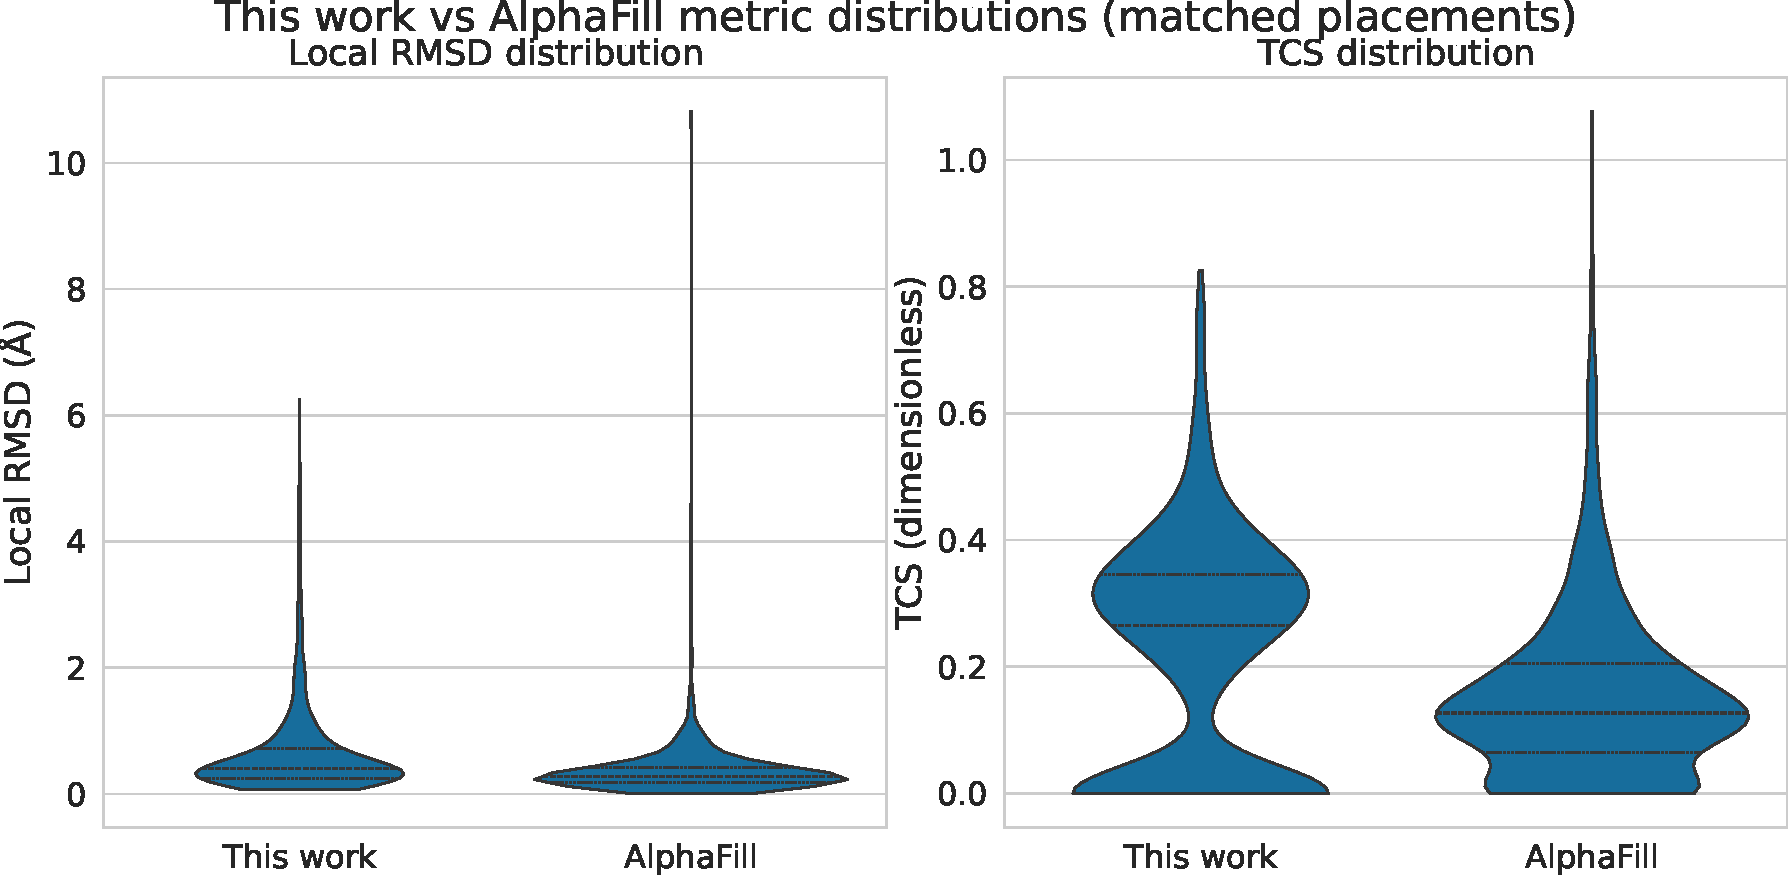
\includegraphics[width=0.9\linewidth]{figures/03_results/fig_ff_af_metric_distributions.pdf}
    \caption[Pipeline vs. AlphaFill distributions]{Distributions of local \gls{rmsd} and \gls{tcs} for this pipeline and AlphaFill on the matched cohort described in Section~\ref{sec:results-external}. Violin plots show quartiles and density for each pipeline.}
    \label{fig:ff-af-dist}
\end{figure}

\begin{figure}[ht]
    \centering
    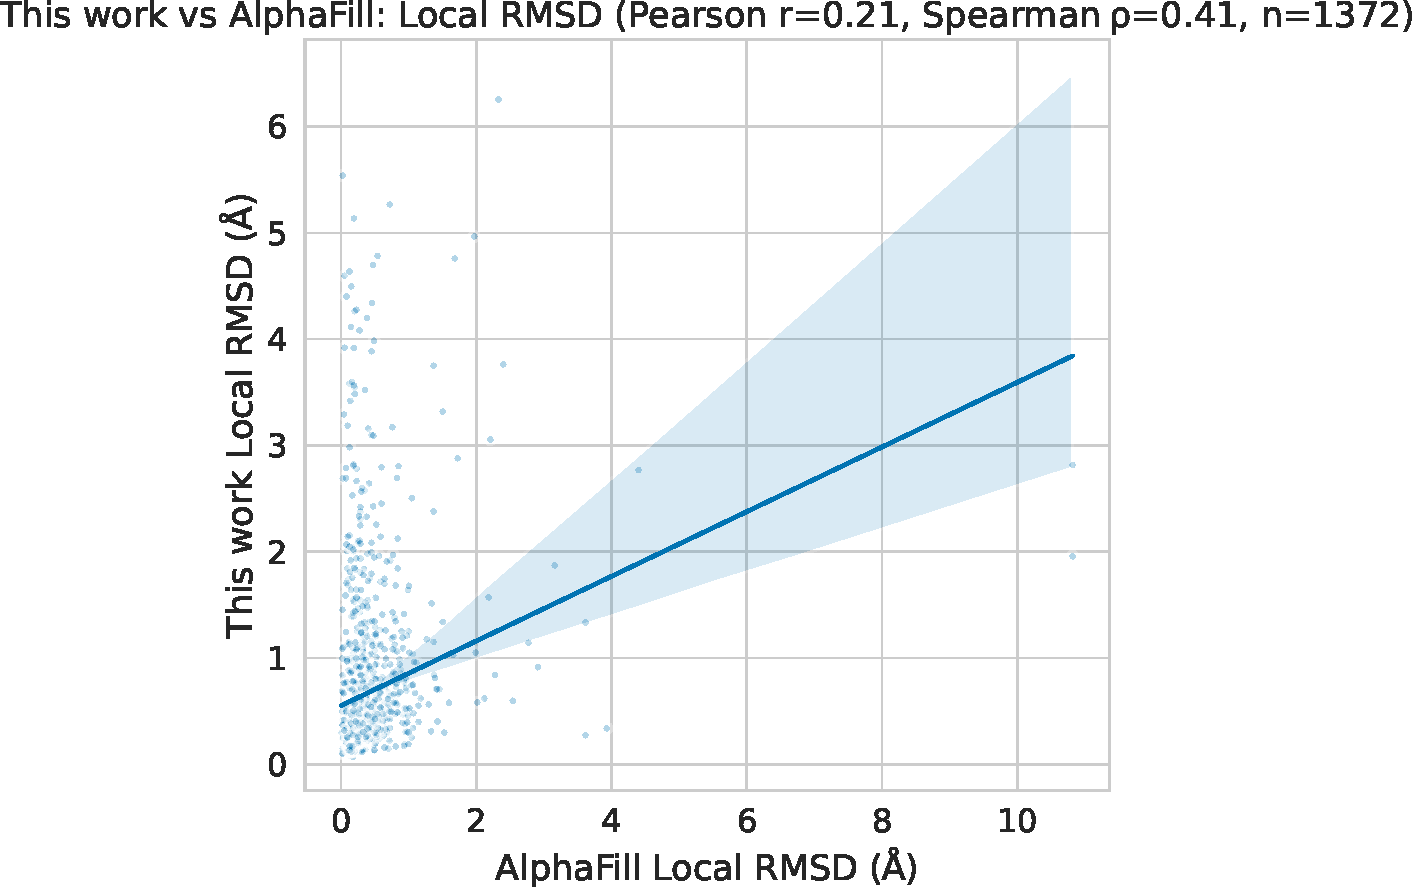
\includegraphics[width=0.49\linewidth]{figures/03_results/fig_correlation_local_rmsd_ff_vs_af.pdf}\hfill
    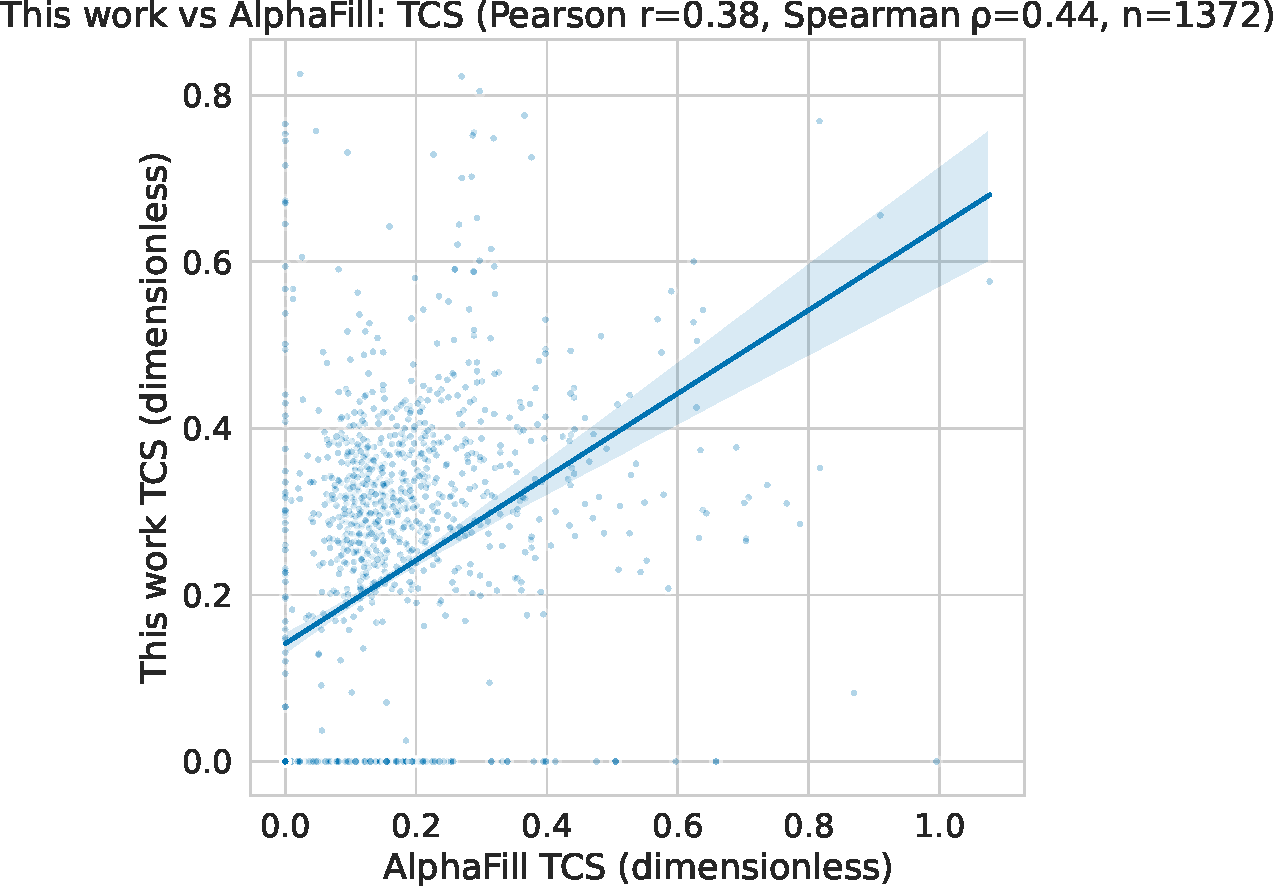
\includegraphics[width=0.49\linewidth]{figures/03_results/fig_correlation_tcs_score_ff_vs_af.pdf}
    \caption[Pipeline vs. AlphaFill correlations]{Correlation of this pipeline (TP) vs.\ AlphaFill (AF) on the matched cohort from Section~\ref{sec:results-external}. The left panel shows local \gls{rmsd} and the right panel shows \gls{tcs}; Pearson $r$ and Spearman $\rho$ with sample sizes are annotated in each title.}
    \label{fig:ff-af-corr}
\end{figure}

\begin{figure}[ht]
    \centering
    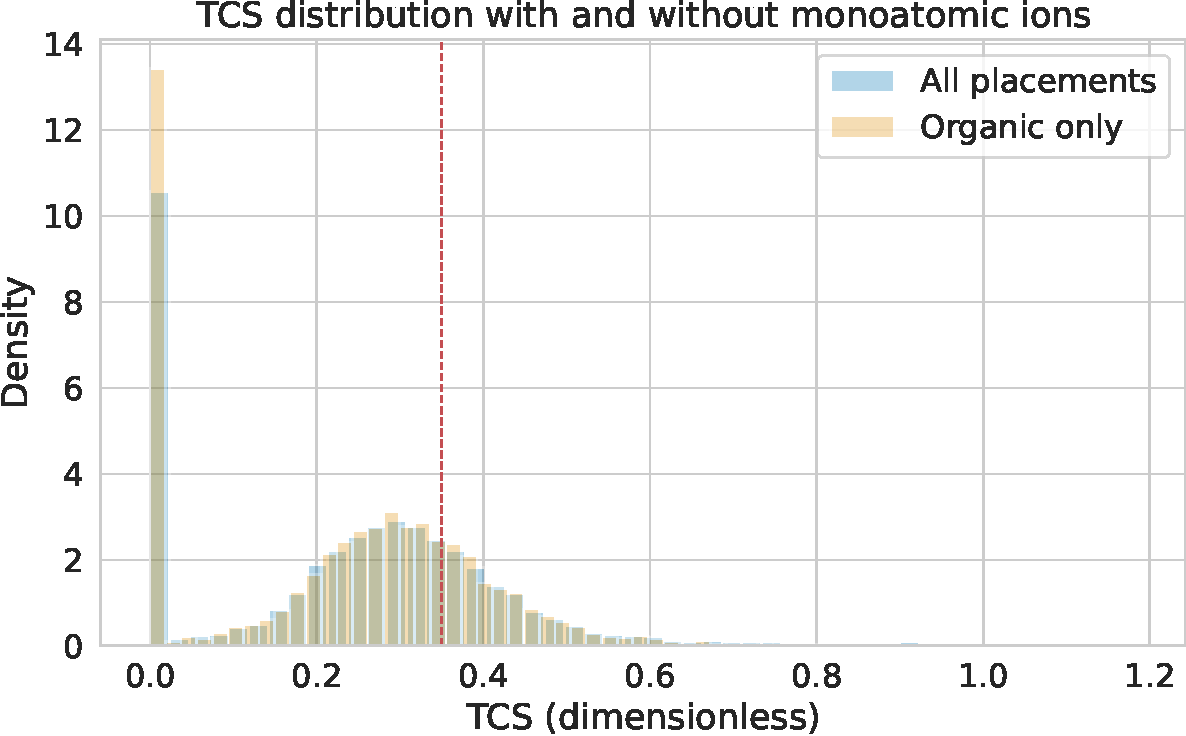
\includegraphics[width=0.75\linewidth]{figures/03_results/fig_tcs_distribution_ion_exclusion.pdf}
    \caption[TCS distributions with ion exclusion]{\gls{tcs} distributions with (blue) and without (green) monoatomic ions. The vertical line marks the \SI{0.35}{} clash threshold used throughout the analysis.}
    \label{fig:ion-exclusion}
\end{figure}


\chapter{Acknowledgements}
My deepest gratitude goes to Prof. Dr. Matthias Rarey for his trust, feedback, and for setting a research environment that encouraged me. In addition I want to thank Prof. Dr. Andrew Torda for taking on the second reviewers position.
I am equally grateful to my supervisor Tim Kuhrt, for his patience, technical guidance, and constructive (and occasional long off-topic) discussions.
I also want to thank my partner for her encouragement, honest perspectives, and for reminding me to stay balanced throughout the thesis journey.
Furthermore, I also acknowledge the use of generative AI tools (OpenAI's ChatGPT) to assist with translations, summarization, ideation, and clarifying background concepts during the preparation of this thesis. All interpretations, analyses, and conclusions presented here remain my own responsibility.

\Assertion
\end{document}
